\graphicspath{{figure/chap4/}}
\chapter{光的偏振}
\section{偏振光概述}
\insertfig{4-1.png}{光的偏振示意图}{0.7}
作为特定波段的电磁波, 光波自然是一种横波. 在光与物质相互作用的过程中, 主要是光波中的电场矢量起作用, 因此把电场矢量称之为光矢量, 其所在的平面与光射线方向正交. 在这个振动平面上光矢量的振动方向对于光的传播方向是不具有轴对称性的, 因此这种不对称现象就被称为偏振. 纵波的振动方向与波的传播方向一致, 从垂直于波传播方向的各个方向去观察纵波都是一致的, 因此偏振是横波区别于纵波的重要标志.

在垂直于光波的传播方向的平面内, 光矢量可能有不同的振动状态, 每种振动状态都可以被称为一个偏振态, 最常见的光的偏振态大致有五种, 我们一一予以介绍.

\insertfig{4-2.png}{光的五种宏观偏振态}{1}

(1)线偏振光. 在观测时间内光矢量的方向始终不变, 如图(a)所示, 其振动可以被表示为:
\[
\bm{E}(t) = \bm{A} \cos\omega t \quad \text{or} \quad E_x(t)=A_x\cos\omega t, \; E_y(t) = \cos(\omega t+\delta)
\]

两个正交振动的相位差$\delta$决定了光的振动象限, 振幅比$\frac{A_y}{A_x}$决定了光矢量的线偏振角.

(2)自然光. 自然光是由大量的不同取向的彼此无关的特殊优越取向的线偏振光构成的. 因此自然光相对传播方向室友轴对称性的, 如图(b)所示. 各种普通光源, 如日光, 钠光灯等均属自然光. 这是因为虽然这些光源在微观持续发光时间$\tau_0$内发射的一段波列是线偏振光, 但是其频率, 相位, 振动方向, 波列长度等均不同, 因此不存在哪个方向相对其他更具优势.

(3)部分(平面)偏振光或称部分线偏振光, 其与自然光的差距仅在于其不具有轴对称性而是具有一个优越方向, 如图(c)所示. 在优越方向上其具有最大的光强. 自然光经界面反射和折射后一部分将会变为部分偏振光. 我们用偏振度描述其偏振程度, 设部分偏振光最大振幅对应的光强为$I_{\max}$, 最小振幅对应的光强为$I_{\min}$, 则我们定义偏振度:
\[
P = \frac{I_{\max}-I_{\min}}{I_{\max}+I_{\min}}
\]

当偏振度为$0$时, 部分偏振光退化为自然光: 当偏振度为$1$时, 部分偏振光退化为线偏振光.

圆偏振光和椭圆偏振光我们会在后面介绍.

下面我们介绍线偏振光的获得.

\insertfig{4-3.png}{偏振片与透振方向}{0.7}

在一张硝化纤维薄膜上敷上一层硫酸碘奎宁超微晶粒, 在拉伸之后, 这些晶粒定向有序排列而固化于这张薄膜上, 形成一张人造偏振片. 偏振片对于入射光的电矢量的吸收有强烈的方向性, 一个方向可以充分地透射, 另一个与其正交的方向上电矢量被强烈地吸收. 我们分别称这两个方向为透振方向和消光方向. 一般而言拉伸方向是消光方向, 透振方向与拉伸方向垂直.

任何一种偏振态的光束, 经过偏振片后都会变成线偏振光. 凡是能够产生线偏振光的期间都被称为起偏振器, 简称起偏器. 用于检验线偏振光的偏振片或者其他起偏器都被称为检偏振器, 简称检偏器.

如前图所示, 我们考虑一个线偏振光透过偏振片. 设线偏振光原有的偏振方向为$A_0$, 其中与透振方向一致的平行分量$A_{\parallel}$可以透过偏振片, 而垂直分量$A_{\perp}$被$P$吸收, 因此透射光强$I_P=A_{\parallel}^2 = A_0^2\cos^2\alpha$. 也就是说:
\[
I_p(\alpha) = I_0\cos^2\alpha
\]
其中$I_0$为入射光强, $\alpha$为入射线偏振光的偏振方向与偏振片透振方向的夹角, 这式子被称为马吕斯定律. 注意这定律仅适用于线偏振光. 马吕斯定律没有考虑偏振片对于光的吸收, 如果设偏振片对于光强的透过率为$\gamma$, 则我们可以给出:
\[
I = \gamma I_0 \cos^2 \alpha
\]

据此, 当一个偏振片$P$, 面对一束入射的线偏振光而旋转时, $\alpha$历经$0 \to 2\pi$的变化, 其光强会出现: 最亮$\to$消光$\to$最亮$\to$消光, 彼此之间间隔为$\frac{\pi}{2}$. 若以一个偏振片作为检偏器, 只有线偏振光在旋转过程中会出现消光的现象.

接下来我们考察自然光和部分偏振光透过偏振片的影响. 对于自然光, 无论偏振片位于何处, 对自然光来说是没有去别的, 其光强按照马吕斯定律以$\cos^2\theta$比率通过, 注意到在一个周期内$\cos^2\theta$的均值为$\frac{1}{2}$, 因此透射光强为入射光强的一半.

\insertfig{4-4.png}{部分偏振光透过检偏器}{0.6}

对于部分偏振光, 当偏振片作为检偏器旋转一周时, 不会出现消光现象, 而是出现一个极小光强. 我们以极大$I_M$和极小光强$I_m$出现时的透振方向构建正交坐标架. 我们可以把构成部分偏振光的大量不同取向的线偏振光分解为两个正交振动, 其光强分别为$I_x=I_m$,$I_y=I_M$, 入射光的总光强为$I_0=I_x+I_y=I_m+I_M$, 因为这两个正交振动是彼此完全不相干的. 因此其他方向的透射光强$I_p(\alpha)$就等于$I_m$,$I_M$按照马吕斯定律在$\alpha$方向贡献的和:
\[
I_p(\alpha) = I_m\cos^2\alpha+I_M\sin^2\alpha= I_m(1-\sin^2\alpha)+I_M\sin^2\alpha = I_m+(I_M-I_m)\cos^2\beta
\]
根据这个光强形式, 我们可以看出其中的第一项类似于自然光透过偏振片的光强, 第二项类似于线偏振光透过偏振片的光强, 因此我们可以说部分偏振光是由光强为$2I_m$的自然光和$I_M-I_m$的线偏振光混合而成的, 线偏振光的偏振方向沿着出现$I_M$的透振方向.

综合以上的讨论, 我们知道了偏振片能够区分自然光, 线偏振光和部分偏振光. 其透过旋转一周的检偏器时出现的现象分别是光强不变, 出现消光现象和出现极小但不为$0$的光强三种.

接下来我们将讨论光在介质界面上发生反射和折射时的偏振现象, 此部分的理论超出了课程的要求, 我们以注记的形式给出一部分, 有兴趣的读者可以自行查阅相关资料.
\begin{noteenv}
    \insertpic{4-5.png}{光在介质界面反射折射的基本图像}{1}

    在这张图中$\bm{k}_1,\bm{k}_1',\bm{k}_2$分别表示入射光, 反射光, 透射光的波矢, $\bm{E}_1$为入射光的电矢量, 其被分解为平行入射面的$\bm{E}_p$和垂直入射面$\bm{E}_s$两个正交分量, 分别称为$p$振动和$s$振动, 也把对应偏振方向的光称为$p$光和$s$光. 当入射光只有$p$光时, 反射和透射光也只有$p$光, $s$光同理, 这也说明了$p$和$s$两个振动确实是彼此独立的.

    历史上, 菲涅耳导出了发生反射和透射时的复振幅反射率和透射率的公式:

\[
\left\{
\begin{aligned}
\tilde{r}_{\mathrm{p}} &= \frac{\tilde{E}'_{1\mathrm{p}}}{\tilde{E}_{1\mathrm{p}}} = \frac{n_2 \cos i_1 - n_1 \cos i_2}{n_2 \cos i_1 + n_1 \cos i_2}= \frac{\tan(i_1 - i_2)}{\tan(i_1 + i_2)}, \\[8pt]
\tilde{r}_{\mathrm{s}} &= \frac{\tilde{E}'_{1\mathrm{s}}}{\tilde{E}_{1\mathrm{s}}} = \frac{n_1 \cos i_1 - n_2 \cos i_2}{n_1 \cos i_1 + n_2 \cos i_2} = \frac{\sin(i_2 - i_1)}{\sin(i_2 + i_1)};
\end{aligned}
\right.
\]

\[
\left\{
\begin{aligned}
\tilde{t}_{\mathrm{p}} &= \frac{\tilde{E}_{2\mathrm{p}}}{\tilde{E}_{1\mathrm{p}}} = \frac{2n_1 \cos i_1}{n_2 \cos i_1 + n_1 \cos i_2}, \\[8pt]
\tilde{t}_{\mathrm{s}} &= \frac{\tilde{E}_{2\mathrm{s}}}{\tilde{E}_{1\mathrm{s}}} = \frac{2n_1 \cos i_1}{n_1 \cos i_1 + n_2 \cos i_2}= \frac{2 \cos i_1 \sin i_2}{\sin(i_2 + i_1)}.
\end{aligned}
\right.
\]

这里的复振幅反射率可能出现负数, 其符号代表着半波损失的出现, 我们也可以自然地看出, 当$n_2>n_1$时, $i_2>i_1$, 此时出现了半波损失, 反之则没有, 且透射光无论何时都不会出现半波损失.

在电磁学的学习中, 我们已经了解到了对于平面电磁波, 我们的光强有如下公式:
\[
I = \langle S \rangle = \frac{1}{2}\sqrt{\frac{\varepsilon}{\mu}E_0^2}
\]
对于光频段, $\mu\approx \mu_0$, 而在第一章中我们已经说明$n=\sqrt{\varepsilon_r}$, 因此电磁波的强度可以被表为:
\[
I \approx \frac{n}{2c\mu_0}E_0^2
\]
因此光强的反射率和透射率可以被表示为:
\[
R_p = r_p^2 , \quad R_s = r_s^2 , \quad T_p = \frac{n_2}{n_1}t_p^2, \quad T_s = \frac{n_2}{n_1}t_s^2
\]

根据上述光强反射率公式, 我们可以给出这样的一个曲线, 在给定折射率的情况下描绘处光强反射率随着入射角的变化曲线.

\insertpic{4-6.png}{光强反射率曲线}{0.8}

由图示可以发现, 反射光束中$s$光的光强反射率随着入射角增大单调上升, 而$p$光的光强反射率先下降到$0$, 而后很快地上升. 这个使得$R_p$为$0$的角度就被称为布儒斯特角.

根据我们之前给出的公式, $i_1+i_2=\frac{\pi}{2}$时$p$光的光强反射率为$0$, 结合折射定律, 我们解出:
\[
\tan i_B  =\frac{n_2}{n_1}
\]
\end{noteenv}
在入射光以布儒斯特角$\tan i_B  =\frac{n_2}{n_1}$入射时, 反射光线恰好与折射光线成一个直角. 此时的反射透射情况可以被总结为: 反射的线偏振光强度很小, 折射的部分偏振光的偏振度很低. 反射光的强度只有入射光的$15\%$, 而经过一次透射的部分偏振光的偏振度只有$8\%$, 因此人们往往采用多个平行玻璃板叠加的方式, 获得偏振度较好的透射偏振光.

\begin{figure}[htbp]
    \centering
    % 第一张图
    \begin{minipage}[b]{0.35\textwidth}
        \centering
        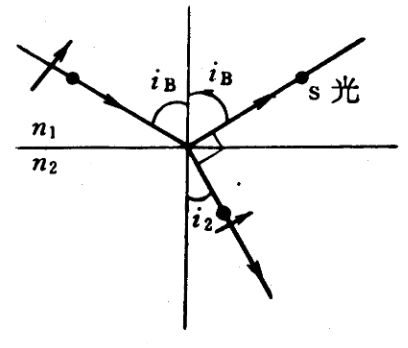
\includegraphics[width=\textwidth]{4-7.png} % figure/image1.png
        \caption{布儒斯特角入射时反射光与折射光正交}
    \end{minipage}
    \hfill
    % 第二张图
    \begin{minipage}[b]{0.64\textwidth}
        \centering
        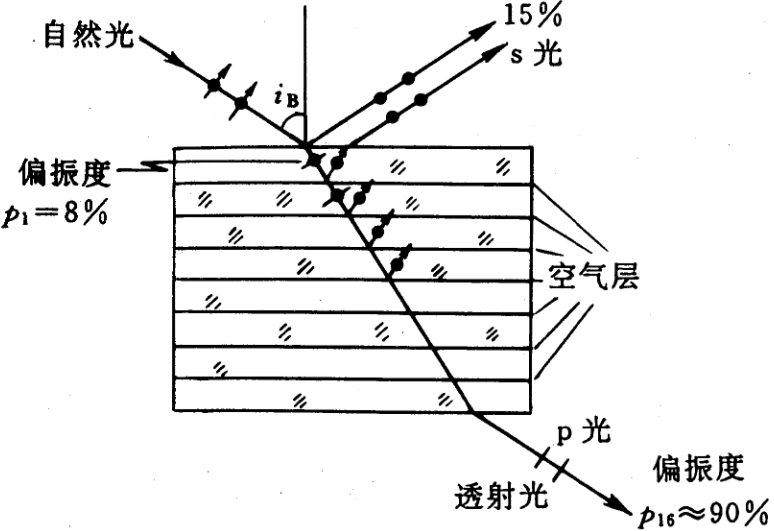
\includegraphics[width=\textwidth]{4-8.png} % figure/image2.png
        \caption{玻片组获取透射偏振光}
    \end{minipage}
\end{figure}


\section{双折射}
晶体是一种各向异性的介质, 固体物理学的晶格几何理论表明, 所有的晶体可以被分为七种晶系, 按照光学性质, 大致可以分为三种.

(1)单轴晶体. 三角晶系, 四角晶系, 六角晶系均系此类. 如方解石, 红宝石, 石英, 冰等等, 常常提到的冰洲石属方解石的一种, 分子式为$CaCO_3$. 其晶胞呈平行六面体形.

(2)双轴晶体. 单斜晶系, 三斜晶系, 正交晶系均系此类. 如蓝宝石, 云母等.

(3)立方晶系. 如$NaCl$晶粒. 它系各向同性介质.

双折射的现象如下所述. 一细光束正入射于一块冰洲石表面, 将有两束光透射出来, 其中一束光沿着入射光方向直接透射, 遵从通常的折射定律, 另一束光从另一高度透射, 这意味着这束光在冰洲石内发生了偏折, 其不遵从通常的折射定律, 这一现象被称为双折射. 遵从通常各向同性介质中折射定律的光称为寻常(ordinary)光, 简称为o光; 不遵从通常折射定律的光, 称为非常(extraordinary)光, 简称为e光.

\insertfig{4-9.png}{双折射现象}{0.45}

若我们的入射光是自然光, 还能进一步发现, 出射的两束透射光是线偏振光, 且偏振方向不相同. 当用一个偏振片去观察两光束时, 一个清晰一个消失, 转过$\frac{\pi}{2}$后恰好反转.

\insertfig{4-10.png}{方解石晶胞与光轴}{0.3}

晶体中存在一个特殊的方向, 光沿着这个方向传播时不发生双折射现象, 这个方向称为晶体的光轴. 冰洲石晶体的光轴方向沿着其两个顿棱角顶点的连线方向. 需注意光轴不是一条线, 而是晶体中的一个特殊方向.

据此, 我们可以引入若干平面. 设一光线以$\bm{r}$入射于晶体表面, 对于一个入射点, 有两个方向值得注意: 晶体表面的法线$\bm{N}_s$和晶体内部的光轴$\bm{z}$. 由$(\bm{N}_s,\bm{z})$组成的平面被称为晶体主截面, 此外还有一个入射面, 其是由$(\bm{N}_s,\bm{r}_1)$组成的平面. 实验上法线, 当入射面与主截面重合时, e光的偏折仍然在入射面内, 而当入射面与主截面不一致时, e光射线就可能不在入射面内. 同时我们定义主平面$(\bm{r},\bm{z})$, 其是由光线和光轴组成的平面.

上面我们介绍了晶体双折射现象. 惠更斯在其著作中提出了一个理论模型, 下面予以介绍.

\insertfig{4-11.png}{双折射的理论解释}{1}

设想单轴晶体内有一个点光源, 如图所示, 其中$\bm{z}$轴方向为晶体光轴方向, 用一系列平行的虚线表示. 沿着任意传播方向$\bm{r}$考察光波的传播行为, 对o光和e光应该分别考虑, 我们定义o光的振动光矢量$\bm{E}_o\perp\text{主平面}(\bm{r},\bm{z})$, e光的振动光矢量$\bm{E}_e\parallel\text{主平面}(\bm{r},\bm{z})$.

o光的振动的传播具有各向同性, 其波前为球面$\sigma_o$, 传播速度为$v_o$, 与传播方向角$\xi$无关. e光的振动传播具有各向异性, e光的传播具有各向异性, 其波前为旋转椭球面, 转轴为光轴$\bm{z}$. 两者的波面相切于光轴, e光的传播速度$v$与方向角$\xi$有关, 其形式为:
\[
v^2 = \frac{v_e^2v_o^2}{v_e^2\cos^2\xi+v_o^2\sin^2\xi}
\]
这公式不需要读者掌握, 但我们可以看出$\xi=0$时, 其传播速度为$v_o$, 也说明了沿着光轴方向上传播不出现双折射现象; $\xi=\frac{\pi}{2}$, 其传播速度为$v_e$. 我们可以引入折射率$n$来表示光速, 与上述$v_o$,$v_e$对应的折射率$n_o$,$n_e$被称为单轴晶体的两个主折射率, 即为:
\[
n_o = \frac{c}{v_o}, \quad n_e =\frac{c}{v_e}
\]
对于其他传播方向, 折射率可以被表示为:
\[
n^2 = n_o^2\cos^2\xi+n_e^2\sin^2\xi
\]
可以看出对于其他传播方向, e光传播速度介于$v_o,v_e$之间, 折射率也介于$n_o,n_e$之间.

根据$v_e>v_o$或者$v_e<v_o$, 可以将晶体划为正负两类. 对于负晶体:
\[
v_e \geq v_e(\xi) \geq v_o , \quad n_e \leq n_e(\xi) \leq n_o
\]
对于正晶体
\[
v_e \leq v_e(\xi) \leq v_o , \quad n_e \geq n_e(\xi) \geq n_o
\]

\insertfig{4-12.png}{正负晶体的波面示意图}{0.6}

简而言之, 对于负晶体, e光为快光, o光为慢光. 反之对于正晶体, o光为快光, e光为慢光.

如果我们关注光矢量与$\bm{z}$的夹角, 我们可以更深刻地理解e光传播的各向异性. 由于e光振动平行于主平面, 故对于不同的传播方向$\xi$, 其光矢量与光轴的夹角$\beta=\frac{\pi}{2}-\xi$也随之改变, $\beta$在$0$到$\frac{\pi}{2}$间取值, 于是e光速度也介于$v_e,v_o$之间. 而o光的光矢量垂直于主平面, 故对于任意的传播方向角, 其与光轴的夹角始终为$\frac{\pi}{2}$, 因此o光的传播具有各向同性. 且在沿着光轴方向时, 两者的光矢量与光轴夹角均为$\frac{\pi}{2}$, 故不出现双折射现象.

若我们知道光在介质或者晶体中的传播速度, 就可以通过惠更斯作图法求得折射光线的方向. 晶体中的惠更斯作图法与我们在第一章第一节中介绍的惠更斯作图法几乎一致, 其区别仅在于界面上的一个点次波源将产生两个次波面进入晶体, 一个是o光次波面, 呈球面; 另一个是e光次波面, 呈旋转椭球面. 相应地会产生两个包络面$\Sigma_o$,$\Sigma_e$, 分别为o光和e光的宏观波面. 下图展示了我们通过惠更斯作图法确定e光射线$\bm{r}_e$和光矢量方向$\bm{E}_e$和o光射线$\bm{r}_o$和光矢量方向$\bm{E}_o$. 这里我们设定了入射面和晶体主截面重合于纸面, 从而各折射光线均位于入射面内.

\insertfig{4-13.png}{晶体中的惠更斯作图法}{1}

我们可以从中得到两个重要结论.

(1)o光射线满足折射定律, e光射线不满足折射定律, 甚至可能出现图4.14中的怪异偏折. 仅当光轴垂直入射面的时候, o光与e光均满足折射定律.

(2)o光射线$\mb{r}_o$总是正交于其波面$\Sigma_o$, 而e光射线$\mb{r}_e$与波面$\Sigma_e$并不一定正交.

\insertfig{4-14.png}{两个结论示意图}{0.6}

我们再考虑两种重要的入射情形.

(1)晶片厚度均匀, 光轴平行表面且光束正入射. 此时不难分析得知, o光和e光的波面平行于晶体表面, 且光射线方向$\mb{r}_o$和$\mb{r}_e$均与波面正交, 而从晶体另一表面正出射. 表观上看并无双折射, 但由于两者在晶体内的传播速度不同, 从而导致两者经过该晶片厚度$d$后, 两者光程不同, 从而使得出射的两个正交光振动之间出现了相位差:
\[
\delta = \frac{2\pi}{\lambda}d(n_e-n_o)
\]
这被应用于制作波晶片, 这是一种检验圆偏振光或椭圆偏振光的元件, 留待后面介绍.

\insertfig{4-15.png}{光轴平行表面且正入射}{0.26}

(2)晶片厚度均匀, 光轴任意取向且光束正入射. 虽然光轴任意取向, 简单分析可以确定此时e光波面仍然平行于晶体表面. 此时体内的e光射线方向$\bm{r}_e$也是倾斜的, 与波面法线方向$\bm{N}_e$并不一致, 而是存在一个分离角$\alpha$:
\[
\alpha = \xi - \theta
\]
这里$\xi$角是传播方向与光轴$\mb{z}$的夹角, $\theta$角指的是波面法线$\mb{N}_e$与光轴$\mb{z}$的夹角.

\insertfig{4-16.png}{光轴任意且正入射}{0.72}

总结一下, 我们在单轴晶体的双折射中, 对于一个入射点我们需要关注的有:

6 个方向: 入射光线方向 $\boldsymbol{r}_1$, 表面法线方向 $\boldsymbol{N}_s$, 晶体光轴方向 $\boldsymbol{z}$, 体内 o 光射线方向 $\boldsymbol{r}_o$, 体内 e 光射线方向 $\boldsymbol{r}_e$, 体内 e 光波面 $\Sigma_e$ 法线方向 $\boldsymbol{N}_e$;

4 个面: 入射面 $(\boldsymbol{r}_1, \boldsymbol{N}_s)$, 晶体主截面 $(\boldsymbol{N}_s, \boldsymbol{z})$, o 光主平面 $(\boldsymbol{r}_o, \boldsymbol{z})$, e 光主平面 $(\boldsymbol{r}_e, \boldsymbol{z})$;

3 个角: $\boldsymbol{r}_e$ 与光轴 $\boldsymbol{z}$ 之夹角 $\xi$, $\boldsymbol{N}_e$ 与光轴 $\boldsymbol{z}$ 之夹角 $\theta$, $\boldsymbol{r}_e$ 与 $\boldsymbol{N}_e$ 之夹角 $\alpha$．

\insertfig{4-17.png}{双折射现象总结}{0.4}

下面我们介绍若干基于双折射现象制作的光学器件. 首先是晶体棱镜. (下面的图中都用虚线标示光轴方向)

晶体棱镜通常是由两块按照一定方式切割下来的晶体三棱镜组合而成. 通过晶体棱镜, 入射的自然光被分解为两束线偏振光, 从空间不同方向出射, 因此晶体棱镜是一种偏振镜, 其可以被用于起偏或者检偏, 其性能优于人造偏振片和玻片堆, 因为晶体双折射现象中o光和e光都是完全的线偏振光. 下面介绍一些经典的晶体棱镜.

\begin{figure}[htbp]
    \centering
    % 第一张图
    \begin{minipage}[b]{0.48\textwidth}
        \centering
        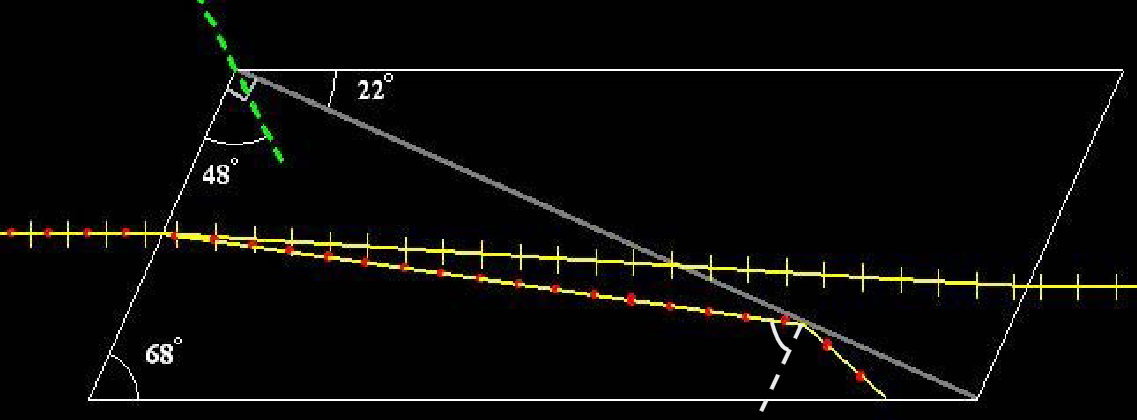
\includegraphics[width=\textwidth]{4-18.png} % figure/image1.png
        \caption{尼科耳棱镜示意图}
    \end{minipage}
    \hfill
    % 第二张图
    \begin{minipage}[b]{0.48\textwidth}
        \centering
        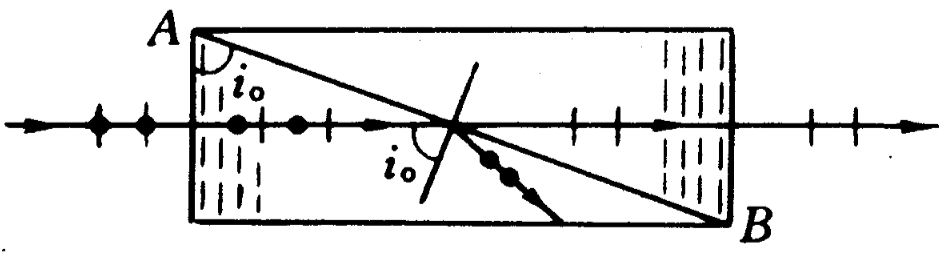
\includegraphics[width=\textwidth]{4-19.png} % figure/image2.png
        \caption{偏振原理示意图}
    \end{minipage}
\end{figure}

(1)尼科耳棱镜. 其由两块方解石棱镜黏合而成, 其光轴平行于两个端面, 常用的粘合剂是加拿大树胶, 其折射率大约为$n_B\approx1.55$, 介于棱镜两个主折射率$n_e\approx 1.4864$和$n_o \approx 1.6584$之间. 在左侧第一块棱镜传播时, 自然光几乎呈现正入射, 表观上虽然不发生双折射, e光和o光分别到达界面$AB$, 对于e光, 其为光疏介质到光密介质, 不可能发生全反射. 全反射是指, 在光由光密介质向光疏介质入射时, 由于折射角的正弦值不能超过1, 从而导致当入射角达到一定大小后, 继续增大入射角, 折射光消失, 所有的光都经由反射传播的现象. 而对于o光来说, 是从光密介质到光疏介质, 将发生全反射, 只要通过合适的调控使得入射角大于临界角. 这样我们就可以从入射光透射的方向获取一束偏振光, 其振动方向平行于主平面或者主截面.


(2)罗雄棱镜. 第一块棱镜光轴垂直棱镜入射面, 第二块棱镜光轴平行表面. 当自然光正入射于第一块棱镜时不发生双折射, 而到达界面后在第二块棱镜中将发生双折射. 这样我们实现了o光和e光的分离, o光会沿着光束垂直前进.

(3)沃拉斯顿棱镜. 其与罗雄棱镜唯一的差别在于, 第一块棱镜的光轴平行于入射表面, 因而其与第二块棱镜的光轴方向正交. 这样一来, 第一块棱镜中的o光, 进入第二块棱镜后变为e光, 其出现的双折射现象导致的空间分离角显著地大于罗雄棱镜.

\insertfig{4-20.png}{罗雄棱镜与沃拉斯顿棱镜}{0.8}

下面我们介绍波晶片.

波晶片是一种产生和检验圆偏振光或者椭圆偏振光的器件, 通常由水晶中切割下来的一个厚度均匀且光轴平行入射表面的薄片构成. 设一束光正入射, 那么表观上不会出现双折射现象, 但是由于横平面上两个特征振动$\mb{E}_o$和$\mb{E}_e$的传播速率不同, 在经过波晶片后会出现相位差, 其结果我们先前已经得到过:
\[
\delta_{oe} = \varphi_o-\varphi_e =\frac{2\pi}{\lambda}d(n_e-n_o)
\]

\insertfig{4-21.png}{波晶片}{0.6}

两种常用的波晶片概述如下. 第一种是四分之一波晶片. 通过其产生的附加相位差服从:
\[
\delta_{oe} = \pm(2k+1)\frac{\pi}{2}, \quad k = 0,1,2\dots
\]

对正晶体, 符号取正, 反之取负. 其提供的有效相位差为:
\[
\delta_{oe} = \pm\frac{\pi}{2}
\]

四分之一波晶片的厚度最小值为:
\[
d_{\min} = \frac{\lambda}{4\Delta n}, \quad \Delta n = |n_e-n_o|
\]

第二种是二分之一波晶片. 通过其产生的附加相位差服从:
\[
\delta_{oe} = \pm(2k+1)\pi, \quad k = 0,1,2\dots
\]

其提供的有效相位差为:
\[
\delta_{oe} = \pi
\]

波晶片的厚度最小值为:
\[
d_{\min} = \frac{\lambda}{2\Delta n}, \quad \Delta n = |n_e-n_o|
\]

波晶片的重要应用是检验和产生圆偏振光和椭圆偏振光. 为此, 有必要对两种偏振光的振动作一介绍.

设波的传播方向沿$z$轴, 则这两种偏振的一般形式可以被写为:
\[
E_x = E_{x0} \cos(\omega t-kz+\varphi_x)
\]
\[
E_y = E_{y0} \cos(\omega t-kz+\varphi_y)
\]

我们定义$\Delta \varphi = \varphi_y-\varphi_x$, 那么当两者振幅相等, 且$\Delta \varphi = \frac{\pi}{2}$时, 其为圆偏振光. 当$\Delta \varphi = 0,\pm \pi$时, 其为线偏振光. $\Delta = \pm\frac{\pi}{2}$时, 为正椭圆偏振光. 其余情况可以参考图4.22.

\insertfig{4-26.png}{相位差带来的不同偏振情况}{0.5}

注意到图中有箭头标注方向, 这代表着偏振光的旋转方向, 可以被分为左旋偏振光和右旋偏振光, 如下图所示.

\begin{figure}[htbp]
    \centering
    % 第一张图
    \begin{minipage}[b]{0.28\textwidth}
        \centering
        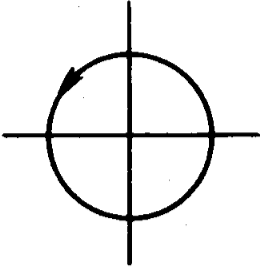
\includegraphics[width=0.5\textwidth]{4-22.png} % figure/image1.png
        \caption{左旋圆偏振光}
    \end{minipage}
    \hfill
    % 第二张图
    \begin{minipage}[b]{0.7\textwidth}
        \centering
        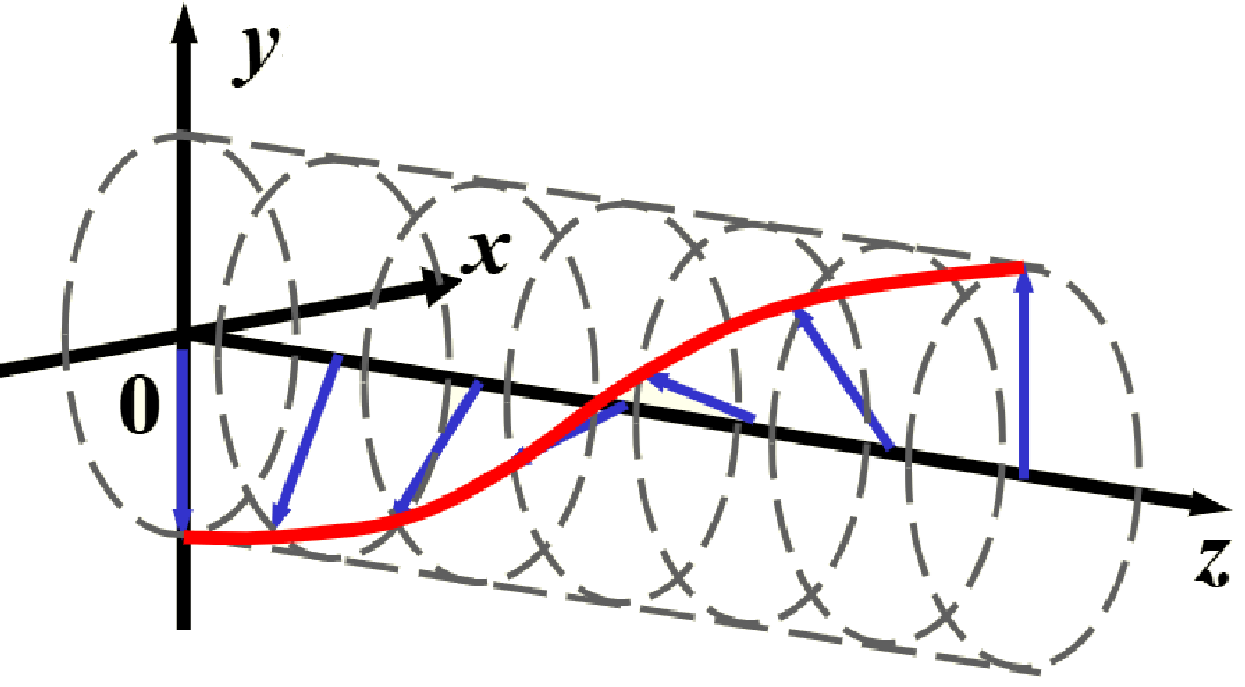
\includegraphics[width=0.6\textwidth]{4-23.png} % figure/image2.png
        \caption{侧视图}
    \end{minipage}
\end{figure}


\begin{figure}[htbp]
    \centering
    % 第一张图
    \begin{minipage}[b]{0.28\textwidth}
        \centering
        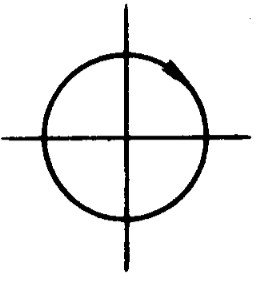
\includegraphics[width=0.5\textwidth]{4-24.png} % figure/image1.png
        \caption{右旋圆偏振光}
    \end{minipage}
    \hfill
    % 第二张图
    \begin{minipage}[b]{0.7\textwidth}
        \centering
        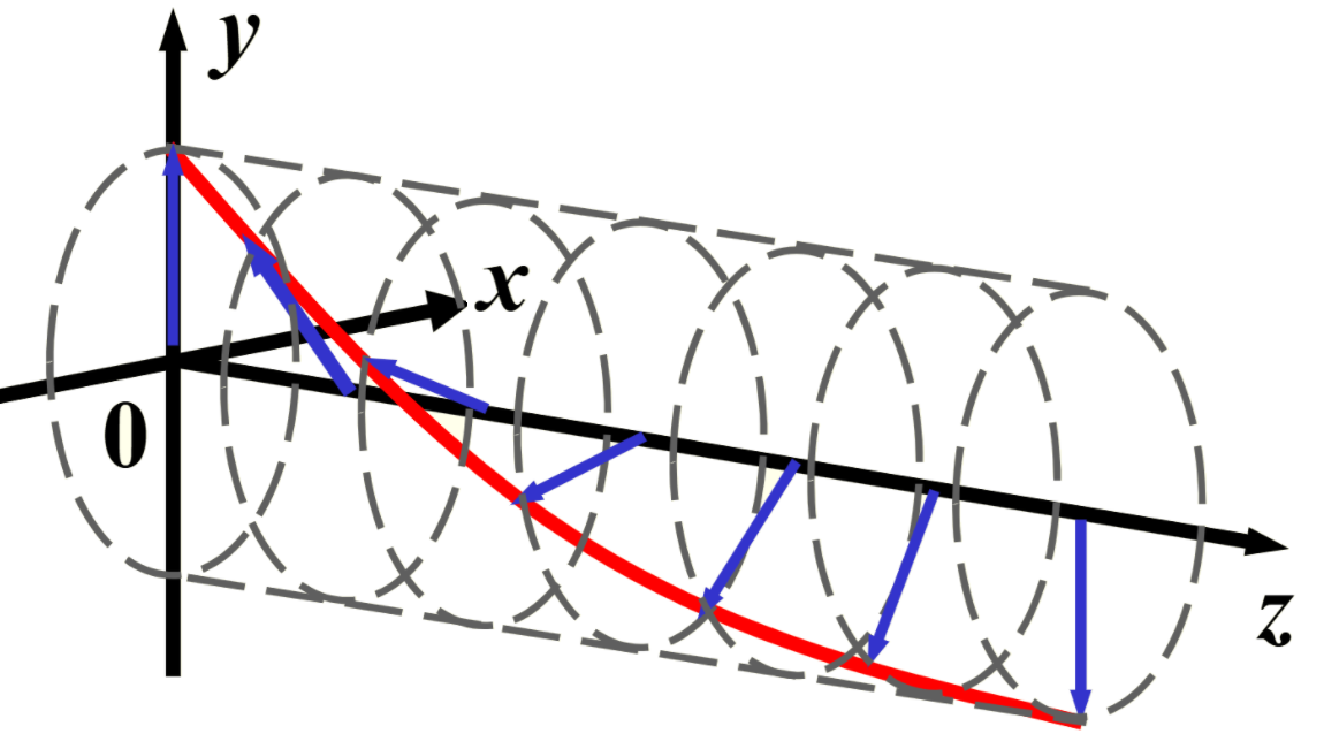
\includegraphics[width=0.6\textwidth]{4-25.png} % figure/image2.png
        \caption{侧视图}
    \end{minipage}
\end{figure}
圆偏振光可以被看作两束振动方向相互垂直, 振幅相等相位差为$\frac{\pi}{2}$的线偏振光构成. 左旋圆偏振光可以被表示为:
\[
E_y = E_0\cos(\omega t-kz), \quad E_x = E_0\cos(\omega t-kz+\frac{\pi}{2})
\]
右旋圆偏振光可以被表示为
\[
E_y = E_0\cos(\omega t-kz), \quad E_x = E_0\cos(\omega t-kz-\frac{\pi}{2})
\]

现在我们介绍如何通过四分之一波片检验圆偏振光与椭圆偏振光.

为此, 我们首先普遍地考察一束偏振光通过波晶片后, 出射光的偏振态. 对于这类问题, 我们以波晶片的光轴方向为基准, 在光束传播的横平面上取定座标架$xy$.$x$轴表示e振动而$y$轴表示o振动. 在此我们取定光轴方向平行e光的振动方向. 接着以此座标架为参考, 确定光束在晶片入射点的相位差$\delta_{oe}$, 再根据波晶片的种类确定附加相位差$\delta'_{oe}$. 最后考察添加相位差之后的出射光的偏振态. 下面我们给出偏振光通过四分之一波片和二分之一波片的一些结果, 见图4.27.值得注意的是, 当入射光的线偏振方位平行或者垂直波晶片光轴时, 出射光仍为线偏振光且偏振方向不变, 因为两个正交振动之一的振幅为0, 不产生附加相位差.

可以观察到, 当线偏振光与光轴的夹角为$\frac{\pi}{4}$时, 将变为圆偏振光; 夹角不为0或者$\pi$时, 将变为正椭圆偏振光. 正椭圆偏振光和圆偏振光将变为线偏振光, 斜椭圆偏振光仍然是斜椭圆偏振光.

\insertfig{4-27.png}{偏振片通过波晶片后的偏振态}{0.8}

在自然光条件下, 如果我们想要获得圆偏振光, 需要一个偏振器和和一个四分之一波片联合作用, 并且需要保证偏振片的透振方向与光轴方向$e$之夹角为$\frac{\pi}{4}$.

\begin{noteenv}
    实际上的偏振片并不会标明其透振方向, 实际上的波晶片也不会标明其光轴方向. 因此我们可以采取下面的实验来确保$\frac{\pi}{4}$夹角的实现.
    \begin{itemize}
        \item 取两个偏振片$P_1,P_2$, 安排在光路中, 转动其中一个直到消光. 此时两偏振片的透振方向正交.
        \item 取一个四分之一波片插入两偏振片之间, 此时一般不再消光. 转动四分之一波片一周, 将出现四次消光状态, 消光时说明四分之一波片的光轴平行或者垂直e光振动方向. 转动四分之一波片直到消光.
        \item 顺或逆时针转动$P_1$经过$\frac{\pi}{4}$角度, 则可以保证透振方向$P_1$与光轴$e$的夹角为$\frac{\pi}{4}$.
    \end{itemize}
\end{noteenv}

使用同样的装置, 可以区分圆偏振光和自然光. 两者的共同特点是偏振度均为0, 且在横平面上的偏振结构具有轴对称性. 取一张偏振片面对两种偏振光转动时, 出射光强始终不变. 为此我们在偏振片前插入一个四分之一波片.

对于圆偏振光, 经过四分之一波片后成为一个线偏振光. 因此转动后面的偏振片, 会出现消光状态. 对于自然光, 其经过四分之一波片后会变为包含大量长短轴比值不同, 彼此不相关的椭圆偏振光的集合, 宏观上看仍有轴对称性, 因此转动偏振片时不发生消光. 这样我们就区分了圆偏振光与自然光.

产生椭圆偏振光时, 只需要将我们在产生圆偏振光时所使用的装置, 把第一个偏振片$P_1$的透振方向调整为非0,$\pi$,$\frac{\pi}{4}$的任意角度, 就可以获得椭圆偏振光.

椭圆偏振光和部分偏振光的共同特点是, 其偏振度介于$(0,1)$之间, 取一张偏振片面对这两者之一转动时, 表现出的变化特点都是有光强的极大和极小, 但无消光. 为此我们仍然在偏振片前插入一张四分之一波片.

对于椭圆偏振光, 当我们调整波片的光轴方向, 使得入射的椭圆偏振光的长短轴方向与波晶片的坐标轴$(o,e)$方向一致时, 入射的椭圆偏振光是一个正椭圆, 经过波片后便成为一个线偏振光, 转动偏振片, 将存在消光现象. 对于部分偏振光, 其经过四分之一波片后出射的是大量椭圆偏振光的集合, 但其宏观特点是相同的, 因此当后面的偏振片转动过程中, 有光强变化, 但是没有消光. 这样我们就区分了椭圆偏振光与部分偏振光.

\begin{noteenv}
    其实验操作可以概述如下:
    \begin{itemize}
        \item 取一偏振片, 安排在光路中, 转动偏振片, 记录光强极大和极小值的角度, 此即为椭圆偏振光的长轴和短轴的角度.
        \item 根据获取圆偏振光中的方法, 找到四次消光状态对应的两个方向, 此即为光轴的两个可能方向, 其应该是彼此垂直的.
        \item 将任意一个可能方向与前述的长轴方向对齐.
    \end{itemize}
\end{noteenv}

总结一下, 我们检验光的偏振态应该遵循下列步骤.

(1)使用一个偏振片, 旋转一周检验有无消光, 若有, 则为线偏振光.

(2)若旋转一周中光强无变化, 则为圆偏振光或自然光; 若光强有极大极小但无消光, 则为部分偏振光或者椭圆偏振光. 此后插入四分之一波片, 按照前述流程区分自然光和圆偏振光或者部分偏振光与椭圆偏振光.

\insertfig{4-28.png}{检验偏振态的流程}{0.5}

\section{偏振光干涉}
\insertfig{4-29.png}{偏振光干涉装置}{0.6}

一个典型的偏振光干涉装置如4.29所示, 我们以自然光入射. $P_1$和$P_2$为两个偏振片, $C$为一光学装置, 一般为波晶片.

我们先介绍一下可能的一些现象.

(1)若波晶片厚度均匀, 单色光入射, 那么在输出屏上光强$I_2$均匀分布, 若转动$P_2$或者其他元件, 则输出光强随之变化.

(2)若波晶片厚度不均匀且单色入射, 那么输出光强呈现不均匀分布, 若转动$P_2$或者其他元件, 强度图样随之发生变化, 每当$P_2$转过$\frac{\pi}{2}$角度, 亮纹与暗纹就交替一次.

(3)若白光入射, 在以上两种情形下, 输出场呈现彩色条纹或图样, 若转动$P_2$或者其他元件, 输出场的色彩分布随之发生变化, 每当$P_2$转过$\frac{\pi}{2}$角度, 两种互补色便交替变化一次. 均匀晶片条件下视场中仍然是均匀的光场.

\insertfig{4-30.png}{求解输出光强}{0.7}

我们对上述现象作一分析. 经过$P_1$后自然光变为线偏振光, 其振幅矢量为$\bm{A}_1$. 进入波晶片后, 齐备分解为两个正交的特征振动, 其振幅矢量分别为$\bm{A}_e$和$\bm{A}_o$. 通过波晶片后, 两个正交的特征振动产生了相位差变化, 记为$\delta'_{oe}$. 而通过$P_2$后光矢量只能是平行于$P_2$透振方向的分量, 因此需要进一步分解而获得两个在同一方向上的振幅矢量$A_{2e}$和$A_{2o}$. 这两个振动满足同频, 稳定相位差且振动方向相同这三个相干条件, 且空间上重叠, 因而会发生干涉.

因此输出光强会被表示为双光束干涉强度的形式:
\[
I_2(x,y)=A_{2e}^2+A_{2o}^2+2A_{2e}A_{2o}\cdot \cos \delta
\]

振幅分量为:
\[
A_{2e}=A_1\cos\alpha\cos\beta, \quad A_{2o} = A_1\sin\alpha\sin\beta, \quad  A_1^2 = \frac{1}{2}I_0
\]
其中相位差$\delta$由三项组成:
\[
\delta = \delta_{oe}(A)+\delta'_{oe}+\delta''
\]
$\delta_{oe}(A)$表示入射波晶片前o光和e光的相位差; $\delta'_{oe}$表示波晶片带来的相位差, $\delta''$表示正交坐标轴向$P_2$投影带来的相位差, 它只有两种可能取值:
\[
\begin{cases}
0, & \text{o, e 投影于 } P_2 \text{ 的方向一致} \\
\pi, & \text{o, e 投影于 } P_2 \text{ 的方向相反}
\end{cases}
\]

考察一些特例: 当$P_1\perp P_2$时, $\alpha+\beta = \frac{\pi}{2}$. 则此时输出光强为:
\[
I_{out} = I_0^2\cos^2\alpha\sin^2\alpha(1+\cos\delta)
\]
且此时$\delta''=\pi$. 当$P_1\parallel P_2$时, $\delta''=0$, 如图4.31, 图4.32所示.

\begin{figure}[htbp]
    \centering
    % 第一张图
    \begin{minipage}[b]{0.46\textwidth}
        \centering
        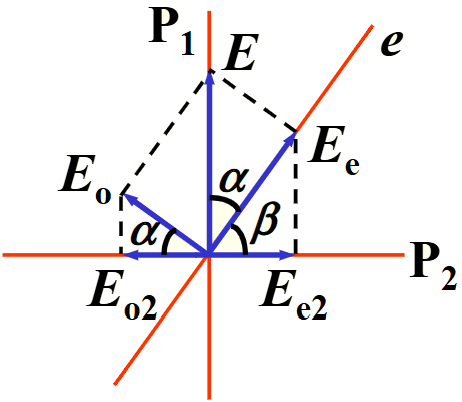
\includegraphics[width=0.75\textwidth]{4-31.png} % figure/image1.png
        \caption{$P_1 \perp P_2$}
    \end{minipage}
    \hfill
    % 第二张图
    \begin{minipage}[b]{0.46\textwidth}
        \centering
        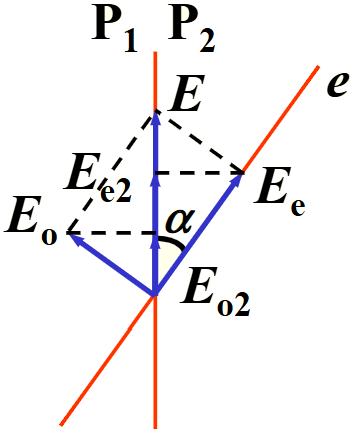
\includegraphics[width=0.625\textwidth]{4-32.png} % figure/image2.png
        \caption{$P_1 \parallel P_2$}
    \end{minipage}
\end{figure}
因此, 我们重新来考察一下这个式子:
\[
I_2(x,y)=A_{2e}^2+A_{2o}^2+2A_{2e}A_{2o}\cdot \cos \delta
\]
我们假定起始状态下:$P_1\perp P_2$, 且$\delta = 2k\pi$, $\alpha=\beta=\frac{\pi}{4}$. 则上述式子可以被化简为:
\[
I_2=(A_{2e}+A_{2o})^2=A_1^2\cos^(\alpha-\beta)
\]
因此, 当我们把$P_2$向光轴方向旋转时, 在$P_2$未越过光轴前, $\delta = 2k\pi$保持不变, 那么光强会逐渐减小. 在$P_2$越过光轴后, $\delta$会产生$\pi$的相位突变, 于是从而使得光强变为:
\[
I_2=A_1^2\cos^2(\alpha+\beta)
\]
在$P_1\parallel P_2$时, 光强将减弱到0.

以上我们讨论的都是单色光的入射. 考虑复色光入射, 注意到波片的所谓四分之一等必须指定光的波长, 因为:
\[
\delta_{oe} = \frac{2\pi}{\lambda}(n_e-n_o)
\]
中包含了波长, 且根据色散理论可能o光和e光的折射率也不尽相同. 因此根据我们上面的讨论, 可能存在一个角度, 使得对于$\lambda_1$波长的光干涉后光强极大, 对$\lambda_2$的光干涉后光强极小, 这样干涉屏上将出现不同颜色的干涉场. 这被称为色干涉.

作为本章的结尾, 我们来讨论杨氏双缝干涉中的偏振光现象.

\insertfig{4-33.png}{杨氏双缝干涉与偏振光}{0.6}

如图所示, 在准单色面光源照明下, 单孔$Q$成为一准单色点光源, 发出自然光, 照明双孔 $(\text{Q}_1, \text{Q}_2)$, 使其成为一对相干点源, 在屏幕上产生一组干涉条纹. 现在, 分别在不同位置插入偏振片 $\text{P}_0$ 或 $(\text{P}_1, \text{P}_2)$ 或 $\text{P}'$, 我们讨论下列条件下屏幕上干涉场的变化.

\begin{enumerate}
    \item [(1)] 仅有偏振片 $\text{P}_0$.
    \item [(2)] 仅有 $(\text{P}_1, \text{P}_2)$, 且 $\text{P}_1 // \text{P}_2$.
    \item [(3)] 仅有 $(\text{P}_1, \text{P}_2)$, 且 $\text{P}_1 \perp \text{P}_2$.
    \item [(4)] 有 $(\text{P}_1, \text{P}_2)$ 和 $\text{P}'$, 且 $\text{P}_1 \perp \text{P}_2$.
    \item [(5)] 有 $\text{P}_0, (\text{P}_1, \text{P}_2)$ 和 $\text{P}'$, 且 $\text{P}_1 \perp \text{P}_2$.
\end{enumerate}

我们可以把自然光分解为两个彼此正交的振动$E_x(t)$ 和 $E_y(t)$, 它们之间是完全非相关的, 即两者的相位差是个随机量, 同理, 由点源 Q 控制的两个点源 $(\text{Q}_1, \text{Q}_2)$ 也是那样, 即 $E_{1x}(t)$ 与 $E_{1y}(t)$ 之间, $E_{2x}(t)$ 与 $E_{2y}(t)$ 之间的相位差是随机量, 但是, $E_{1x}(t)$ 与 $E_{2x}(t)$ 之间, $E_{1y}(t)$ 与 $E_{2y}(t)$ 之间的相位差是稳定的. 据此, 我们对原先无任何偏振片时, 杨氏实验干涉条纹的生成机制可认为是: 最终出现于屏幕上的是这两套分布完全相同的干涉条纹的非相干叠加, 亮纹亮度相较于仅有一组时增加了一倍.

若只有偏振片 $\text{P}_0$, 这相当于只保留了上述一套干涉条纹, 亮纹亮度减弱为一半. 或者说, 因为有了 $\text{P}_0$, 只提取了自然光总光强的一半进入干涉系统, 致使后场的所有光强效应也减弱一半.

若仅有 $(\text{P}_1, \text{P}_2)$, 且 $\text{P}_1 // \text{P}_2$, 亮纹亮度减弱一半; 若 $\text{P}_1 \perp \text{P}_2$, 单凭正交振动必定是非相干叠加这一条, 就可以断定屏幕上亮度均匀, 干涉条纹消失.

那么, 在 $\text{P}_1 \perp \text{P}_2$ 条件下, 若在屏幕前面加一偏振片 $\text{P}'$, 以提取两个振动方向一致的成分, 是否就可以发生相干叠加而生成干涉条纹呢? 实验结果显示, 屏幕上亮度依然均匀而无干涉条纹. 这时, 同频同振动方向这两条相干条件, 虽然得以保证, 但稳定相位差这一条件未能实现, 因为从 $\text{P}_1, \text{P}_2$ 透射过来的是自然光的两个正交振动, 比如 $E_{1x}(t), E_{2y}(t)$, 两者之间的相位差是一随机量, 即使各自向 $\text{P}'$ 投影获得同方向的两个分量, 其间相位差显然还是随机量, 不满足相干条件. 这一现象就是历史上著名的阿拉戈偏振光干涉实验所显示的, 他于 1816 年发现, 从自然光中提取的偏振方向互相垂直的两束光不干涉, 即使外加一偏振片在其交叠区中.

在 $\text{P}_1 \perp \text{P}_2$ 条件下, 若要出现干涉条纹, 必须在前面插入一偏振片 $\text{P}_0$ 于 Q 处, 在后面再插入一偏振片 $\text{P}'$ 于屏幕前. 前者为了保证有稳定的相位差, 因为线偏振光的两个正交分量之间相位差是固定的.

